\documentclass[a4paper,11pt,fleqn]{jarticle}
\usepackage[dvipdfmx]{graphicx}
\usepackage{float}
\usepackage{amsmath}
\usepackage{fancyhdr}

\def \vec#1{\mbox{\boldmath $#1$}} %ベクトルマクロ
\def \bun#1#2{\left(\frac{#1}{#2}\right)} %括弧つき分数マクロ
\def \rot{\nabla \times} %rot
\def \div{\nabla \cdot} %div
\def \intt{\int\!\!\!\int} %2重積分
\def \inttt{\int\!\!\!\int\!\!\!\int} %3重積分

% ページレイアウト
\setlength{\topmargin}{10mm}
  \addtolength{\topmargin}{-1in}
\setlength{\oddsidemargin}{30mm}
  \addtolength{\oddsidemargin}{-1in}
\setlength{\textwidth}{150mm}
\setlength{\textheight}{250mm}
\setlength{\headsep}{2zw}
\setlength{\headheight}{2zw}
\setlength{\topskip}{15mm}
\linespread{1.0}

% サブセクションを1.,2.にする設定
\renewcommand{\thesubsection}{\arabic{subsection}.}

% サブサブセクションを(1),(2)にする設定
\renewcommand{\thesubsubsection}{(\arabic{subsubsection})}

% 大問2の3番目の計算式のラベルを(2.3)にする設定
% 計算式の参照には\eqref{eq:hoge}を使う
\makeatletter
  \renewcommand{\theequation}{\arabic{subsection}.\arabic{equation}}
  \@addtoreset{equation}{subsection}
\pagestyle{fancy}
% ヘッダーの設定
  \lhead[物理数学 2016.04.28]{\leftmark}
  \rhead[\leftmark]{物理数学 2016.04.28}
\renewcommand{\headrulewidth}{0pt}
\makeatother



\begin{document}


\begin{center}
\begin{Large}
演習問題その8  常微分方程式(3)解答例
\end{Large}
\end{center}

\subsection{}
次の1階高次の微分方程式を解け.ただし、$dy/dx=y'$とする.
\begin{eqnarray*}
y=xy'-{y'}^2/4
\end{eqnarray*}
\begin{eqnarray*}
(解答例)
\end{eqnarray*}
クレローの微分方程式。$p=y'$として$x$で微分すれば、
\begin{eqnarray*}
p=p+xp'-\frac{pp'}{2}\Rightarrow p'\left(x-\frac{p}{2}\right)=0
\end{eqnarray*}
まず、$p'=0$のとき、
\begin{eqnarray*}
y=c_1x+c_2
\end{eqnarray*}
また、$x-p/2=0\Rightarrow p=2x$のとき、
\begin{eqnarray*}
y=x^2
\end{eqnarray*}
よって、一般解$y=cx-c^2/4$、特別解$y=x^2$.

\newpage
\subsection{}
次の微分方程式の一般解を求めよ.
\subsubsection{$y''+4y=x$}
(解答例)\\
特解の形を$y_p=Ax+B$として、もとの微分方程式に代入すると
\begin{eqnarray*}
4Ax+4B=x
\end{eqnarray*}
となるので$A=1/4$, $B=0$。よって特解は$y_p=(1/4)x$. 
次に斉次方程式の一般解は$y_0=c_1\cos{2x}+c_2\sin{2x}$となるので一般解は、
\begin{eqnarray*}
y=y_0+y_p=(1/4)x+\cos{2x}+c_2\sin{2x}
\end{eqnarray*}

\subsubsection{$y''-5y'+6y=e^{-x}$}
(解答例)\\
特解の形を$y=Ae^{-x}$として、もとの微分方程式に代入すると
\begin{eqnarray*}
12Ae^{-x}=e^{-x}
\end{eqnarray*}
となるので$A=1/12$となり、特解は$y_p=(1/12)e^{-x}$。
次に同次方程式の特性方程式は$\lambda^2-5\lambda+6=0$となるのでその解は$\lambda=2, 3$である。
よって$y_0=c_1e^{2x}+c_2e^{3x}$となるので一般解は、
\begin{eqnarray*}
y=y_0+y_p=y=(1/12)e^{-x}+c_1e^{2x}+c_2e^{3x}
\end{eqnarray*}

\newpage
\subsection{}
次の高階線形微分方程式を解け.
\subsubsection{$y'''+y''-21y'-45y=0$}
(解答例) \\
特性方程式は
\begin{eqnarray*}
\lambda^3+\lambda^2-21\lambda-45=0 \ 
\Leftrightarrow \ (\lambda+3)^2(\lambda-5)=0.
\end{eqnarray*}
この特性方程式の解は、$\lambda=-3\mbox{(重解), \ 5}$ \\
よって与えられた微分方程式の解は、$C_1, \ C_2, \ C_3$を定数として
\begin{eqnarray*}
y=(C_1x+C_2)e^{-3x}+C_3 e^{5x}.
\end{eqnarray*}

\subsubsection{$y'''+y''-5y'+3y=0$}
(解答例)\\
$y=e^{\lambda x}$として代入すると、特性方程式は
\begin{eqnarray*}
\lambda^3+\lambda^2-5\lambda+3 &=& (\lambda-1)^2(\lambda+3) \\
&=& 0 \\
\Leftrightarrow \lambda &=& 1 (重解) \; , \; -3.
\end{eqnarray*}
よって一般解は、$C_1,C_2,C_3$を定数として
\begin{eqnarray*}
y=(C_1x+C_2)e^{x}+C_3e^.
\end{eqnarray*}


\newpage
\subsection{}
次の微分方程式を解け.
\subsubsection{$y=x(y'+1)+y'$}
(解答例)\\
ラグランジュの微分方程式
$ y = xg(p) + f(p)$,
$p = y'$
の$g(p)=p+1,\ f(p)=p$にあたる。($p = y^{\prime}, \  p'=dp/dx $とする。)
\\
全体を$x$で微分すると、
 \begin{eqnarray*}
  p&=& p+1 + xp' + p' \\
  \Leftrightarrow \ p' &=& -\frac{1}{x+1},  \\
  \ p &=& -\ln{|x+1|} + C. \qquad (C=const.)  …(1)
 \end{eqnarray*}
 これを与式に代入して、
 \begin{eqnarray*}
  y &=& x(- \ln{|x+1|+C+1} )+(- \ln|x+1| +C), \\
  \ y &=& -(x+1)\ln{|x+1|}  + (C+1) x+C.
 \end{eqnarray*}
※(1)式で、$y' = -\ln |x+1| + C$を積分した場合、任意定数が更に出てきて、2つとなる。しかし、本問題は、1階の常微分方程式であるから、任意定数は「1つだけ」。($n$階微分方程式の任意定数は$n$個となる。)
2つ出てきた場合は与式を満たすように片方の定数を与え直す必要がある。そのため、$p = y'$を(1)で求めたら、それを積分せず、そのまま与式に代入して解を求めた方が楽で間違いも起きない。
\subsubsection{$y=x{y'}^2+{y'}^2$}
(解答例)\\
$p=y'$として、$x$で微分すると、
\begin{eqnarray*}
 p &=& p^2 + 2xpp' + 2pp' \\
 \Leftrightarrow 0 &=& p\{ 2(x + 1)p' + p-1 \}.
\end{eqnarray*}
$p=0$のとき、与式から$y=0$となる。\\
$2(x + 1)p' + p-1=0$のとき、これを変形して
\begin{eqnarray*}
 \frac{dp}{p-1} &=& - \frac{dx}{2(x+1)} \\
 \Leftrightarrow \ \log{|p-1|} &=&  -\frac{1}{2}\log{|x+1|} + C_1, \quad (C_1=const.)\\
 \Leftrightarrow \ p &=&  e^{C_1}(x+1)^{-1/2} + 1. 
\end{eqnarray*}
これを与式に代入して、
\begin{eqnarray*}
 y &=& (x+1) (e^{C_1}(x+1)^{-1/2} + 1)^2 \\
 &=& (x+1) (e^{2C_1}(x+1)^{-1} + 2e^{C_1}(x+1)^{-1/2} + 1),\\
 \ y &=& 2C(x+1)^{1/2} + x + 1 + C^2. \quad \left( C=e^{C_1} \right)
\end{eqnarray*}
一般解$y=2C(x+1)^{1/2} + x  +C^2+ 1$, 特異解$y=0$。\\

\newpage
\subsection{}
$p=y'$とおいて階数の引き下げを行うことにより、次の微分方程式を解け.
\subsubsection{$xy''-3y'=0$}
(解答例)\\
$y$を含まない高階の微分方程式。$y'=p$とおくと$xp'-3p=0$。積分して
\begin{eqnarray*}
\int\frac{dp}p &=& 3\int\frac{dx}x+C, \;\;(Cは積分定数)\\
\ln|p| &=& 3\ln|x|+C \\
\Leftrightarrow y'=p &=& C'x^3. \;\;\;\; (C'=\pm e^C とした)
\end{eqnarray*}
$y'=C'x^3$をもう1回積分し、$C_1=C/4,C_2$を定数とすると
\[\hspace{-3cm}
y=C_1x^4+C_2.
\]

\subsubsection{$x^2y''=2xy'+x^2$}
(解答例)\\
$y$を含まない高階の微分方程式。$y'=p$とおくと$x^{2}p'=2xp+x^{2}$である。左辺の$x^{2}$を0とした斉次方程式の一般解は$Cx^{2}$($C$は定数)であり、また、与えられた方程式の特殊解として$-x$がある。よって、与えられた方程式の一般解は
\begin{eqnarray*}
p=Cx^{2}-x.
\end{eqnarray*}
$p=dy/dx$であるから
\begin{eqnarray*}
y=C_{1}x^{3}-\frac{1}{2}x^{2}+C_{2}(C_{1},C_{2}は定数)
\end{eqnarray*}

\newpage
\subsection{}
次の高階同次形の微分方程式を解け.
\subsubsection{$x^2y''+xy'+3y=0$}
(解答例)\\
$F(y,y'x,y''x^2) = 0$であるから、$x = e^u$とおくと、
\begin{eqnarray*}
y' &=& \frac{dy}{du} \frac{du}{dx} = e^{-u}\frac{dy}{du},\\
y'' &=& -e^{-u}\frac{du}{dx}\frac{dy}{du} + e^{-u}\frac{d^2y}{du^2}\frac{du}{dx}
=e^{-2u}\left(\frac{d^2y}{du^2}-\frac{dy}{du}\right).
\end{eqnarray*}
$x = e^u$に注意して代入すれば
\begin{eqnarray*}
x^2y''+xy'+3y = x^2e^{-2u}\left(\frac{d^2y}{du^2}-\frac{dy}{du}\right) + xe^{-u}\frac{dy}{du} + 3y = \frac{d^2y}{du^2} + 3y.
\end{eqnarray*}
よって微分方程式$\frac{d^2y}{du^2} + 3y = 0$を解けば、
\begin{eqnarray*}
y = c_1\sin(\sqrt{3}u + c_2) .
\end{eqnarray*}
$u=\ln x$となるので
\begin{eqnarray*}
y = c_1\sin(\sqrt{3}\ln x + c_2) .
\end{eqnarray*}
ただし$c_1,c_2$は任意定数。

\subsubsection{$yy''-{y'}^2-6xy^2=0$}
(解答例)\\
$y = e^u$とおくと、
\begin{eqnarray*}
y' &=& u'e^{u},\\
y'' &=& (u''+u'^{2})e^{u}.
\end{eqnarray*}
これらを元の式に代入すると
\begin{eqnarray*}
e^{2u}(u''+u'^{2})-e^{2u}u'^{2}-6xe^{2u}=0
\end{eqnarray*}
すなわち
\begin{eqnarray*}
u''=6x
\end{eqnarray*}
これを積分すると
\begin{eqnarray*}
u=x^{3}+C_{1}x+C_{2} (C_{1},C_{2}は定数)
\end{eqnarray*}
したがって
\begin{eqnarray*}
y=e^{x^{3}+C_{1}x+C_{2} }(C_{1},C_{2}は定数)
\end{eqnarray*}

\newpage
\subsection{$+\alpha$問題}
\subsubsection{単振り子}
振り子の最下点からの円弧に沿った長さを$s$をすると、
単振り子の運動方程式は、
\begin{eqnarray*}
m\frac{d^2s}{dt^2}=-mg\sin\theta\sim-mg\frac{s}{l}
\end{eqnarray*}
ここで$\theta\ll1$である。ある時刻tにおける変位s(t)を求めよ。
ここで$t=0$のときの質点は最下点$s=0$で速度$v_0$とする。\\
(解答例)\\
$\frac{d^2s}{dt^2}=-\frac{g}{l}s$の特性方程式は
\begin{eqnarray*}
\lambda^2+\frac{g}{l}=0
\end{eqnarray*}
より、$\lambda=\pm{i}\sqrt{\frac{g}{l}}$. よって、一般解は
\begin{eqnarray*}
s(t)=A\sin{\sqrt{\frac{g}{l}}t}+B\cos{\sqrt{\frac{g}{l}}t}
\end{eqnarray*}
$t=0$の時に最下点$(s=0)$で速度$v_0$より、
\begin{eqnarray*}
s(t)=v_0\sqrt{\frac{l}{g}}\sin{\sqrt{\frac{g}{l}}t}
\end{eqnarray*}
これは振幅$v_0\sqrt{\frac{l}{g}}$、周期$T=\frac{2\pi}{\omega}=2\pi\sqrt{\frac{l}{g}}$の振り子の振動を表す.\\

\newpage
\subsubsection{強制振動}
\begin{eqnarray*}
\frac{d^2y}{dt^2}+\omega_0^2y=F\cos{\omega{t}}
\end{eqnarray*}
は固有角周波数$\omega_0$の振動子に外力$F\cos{\omega{t}}$を加えたときの振動子の運動を記述する方程式である。このとき、以下の問いに答えよ。
\begin{description}
\item[(1)]$\omega\neq\omega_0$の場合の微分方程式の一般解を求めよ。
(解答例)\\
三角関数は二回微分するともとに戻る性質があるから、与えられた微分方程式の特解として
\begin{eqnarray*}
y_p(t)=A\cos{\omega{t}}
\end{eqnarray*}
の形が予想される. これをもとの微分方程式に代入すると、
\begin{eqnarray*}
(-\omega^2+\omega_0^2)A\cos{\omega{t}}=F\cos{\omega{t}}\\
\  A=\frac{F}{\omega_0^2-\omega^2}
\end{eqnarray*}
よって、特解は
\begin{eqnarray*}
y_p(t)=\frac{F_0}{\omega_0^2-\omega^2}\cos{\omega{t}}
\end{eqnarray*}
となる。一方で、与式の斉次解は
\begin{eqnarray*}
y_0(t)=C_1\cos{\omega_0{t}}+C_2\sin{\omega_0{t}}
\end{eqnarray*}
と表せるので、与式の一般解は、
\begin{eqnarray*}
y(t)&=&y_0(t)+y_p(t)\\
     &=&C_1\cos{\omega_0{t}}+C_2\sin{\omega_0{t}}+\frac{F_0}{\omega_0^2-\omega^2}\cos{\omega{t}}
\end{eqnarray*}

\item[(2)]$\omega=\omega_0$の場合の微分方程式の一般解を求めよ。
(解答例)\\
与えられた微分方程式の特解として、
\begin{eqnarray*}
y_p(t)=At \cos \omega_{0}t + Bt \sin \omega_{0}t
\end{eqnarray*}
を仮定する($\omega=\omega_{0}$のとき、$y_p(t)=A \cos \omega_{0}t + B\sin \omega_{0}t$とすると斉次解と一致してしまう)。
これより
\begin{eqnarray*}
y_p'(t)=A \cos \omega_{0}t - At\omega_{0} \sin \omega_{0}t+ B \sin \omega_{0}t+ Bt\omega_{0} \cos \omega_{0}t
\end{eqnarray*}
\begin{eqnarray*}
y_p''(t)&=&-2A \omega_{0}\sin \omega_{0}t - At\omega_{0}^{2} \cos \omega_{0}t + 2B \omega_{0} \cos \omega_{0}t -Bt\omega_{0}^{2} \sin \omega_{0}
\end{eqnarray*}
これらを与えられた式に代入すると
\begin{eqnarray*}
-2A\omega_{0} \sin \omega_{0}t +2B\omega_{0}\cos \omega_{0}t = F\cos \omega_{0}t
\end{eqnarray*}
よって
\begin{eqnarray*}
A=0, B= \frac{F}{2\omega_{0}}
\end{eqnarray*}
よって、特殊解は
\begin{eqnarray*}
y_{p}(t)=\frac{F}{2\omega_{0}}t\sin \omega_{0}t
\end{eqnarray*}
また、与えられた式の斉次解は
\begin{eqnarray*}
y_{0}(t)=C_{1} \cos \omega_{0}t + C_{2}\sin \omega_{0}t
\end{eqnarray*}
で表されるので、与えられた方程式の一般解は
\begin{eqnarray*}
y(t)&=&y_0(t)+y_p(t)\\
     &=&C_{1} \cos \omega_{0}t + C_{2}\sin \omega_{0}t +\frac{F}{2\omega_{0}}t\sin \omega_{0}t
\end{eqnarray*}
参考までに、$t=0$で$y(t)=0,v(t)\equiv dy(t)/dt =0$となる解を考えると
\begin{eqnarray*}
y(t)=\frac{F}{2\omega_{0}}t\sin \omega_{0}t
\end{eqnarray*}
となり、このグラフを描くと下図のように、時間ととともに振幅が増大する(共鳴)。\\
\begin{figure*}[htbp]
\begin{center}
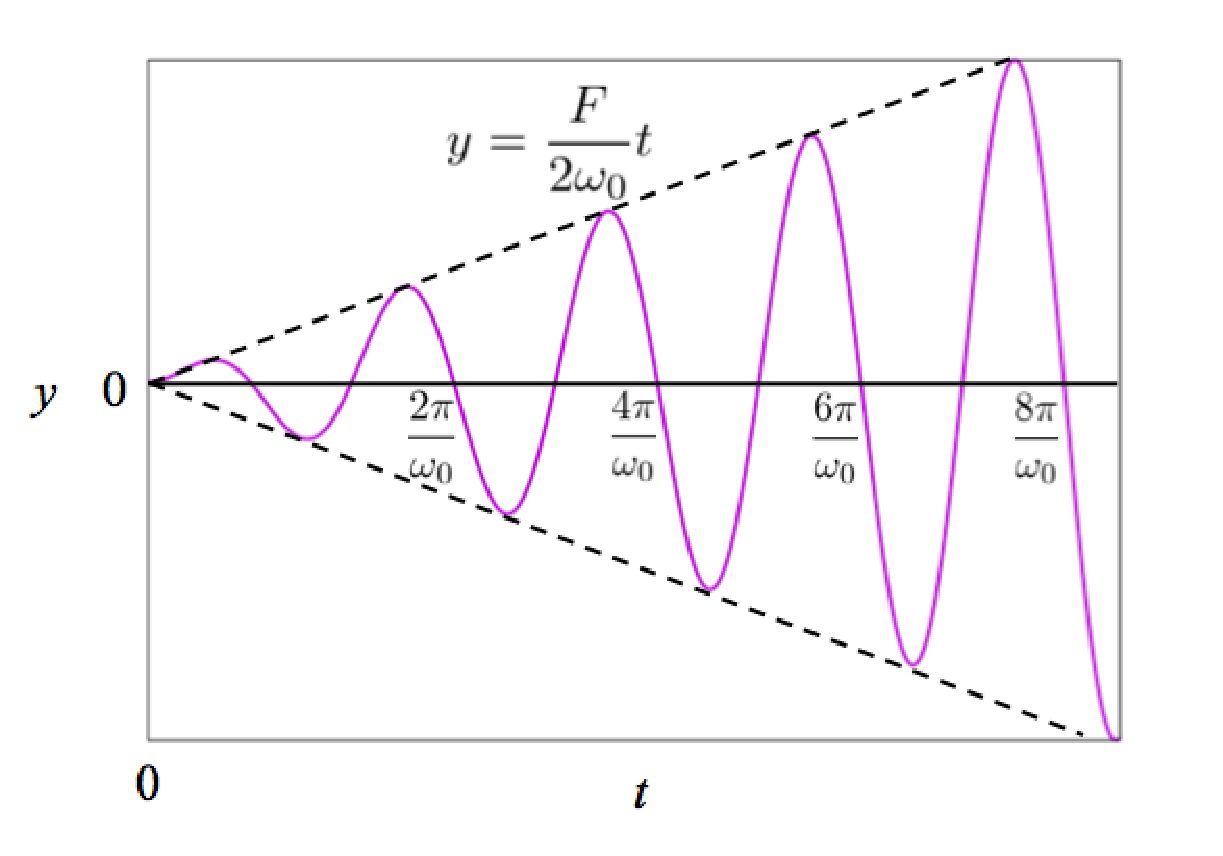
\includegraphics[height=5.5cm,keepaspectratio]{kyoumei.eps}
\label{fig:kyoumei}
\end{center}
\end{figure*}
\end{description}


\end{document}